\documentclass{article}
\usepackage{graphicx} % Required for inserting images

\title{Group 5 lab 4 report}
\author{Ashley Björs,Elliot Bodin,Daniel Rytenberg,Jonas Gerne}
\date{January 2024}

\begin{document}
\maketitle

\section{LUT list}
\begin{figure}[h]
    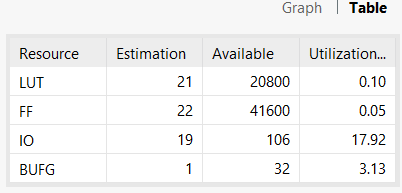
\includegraphics[width=5cm]{{images/Lut1.png}}
    \centering
    \caption{This is the LUT list of step 1}
\end{figure}
\begin{figure}[h]
    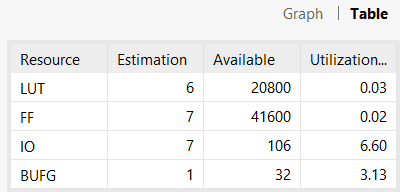
\includegraphics[width=5cm]{{images/Lut2.png}}
    \centering
    \caption{This is the LUT list of step 2}
\end{figure}
   
\begin{figure}[h]
    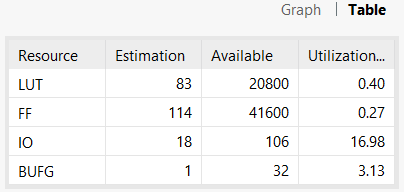
\includegraphics[width=5cm]{{images/Lut3.png}}
    \centering
    \caption{This is the LUT list of step 3}
\end{figure}
\begin{figure}[h]
    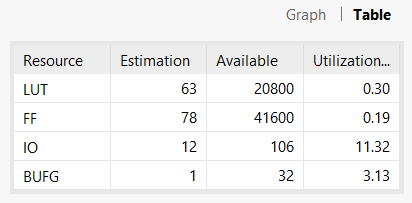
\includegraphics[width=5cm]{{images/Lut4.png}}
    \centering
    \caption{This is the LUT list of step 4}
\end{figure}
              
\clearpage

\section{Waveforms}

\begin{figure}[h]
    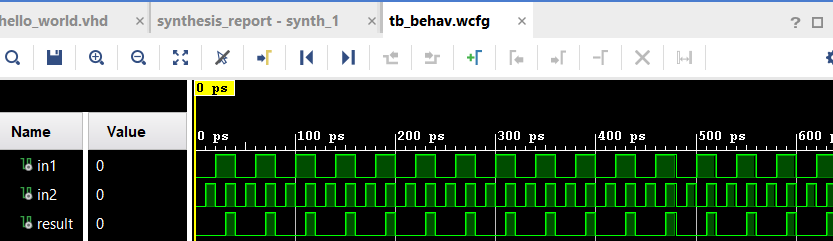
\includegraphics[width=13cm]{{images/sim_step1.png}}
    \centering
    \caption{This is the simulation of step 1}
\end{figure}

\begin{figure}[h]
    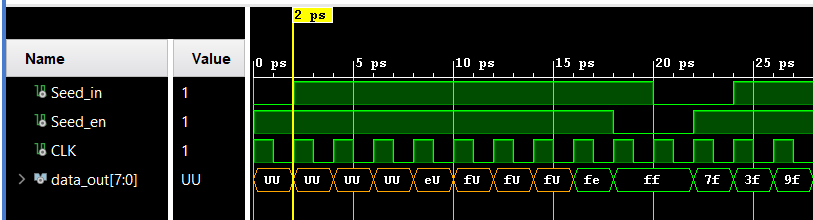
\includegraphics[width=13cm]{{images/sim_step2.png}}
    \centering
    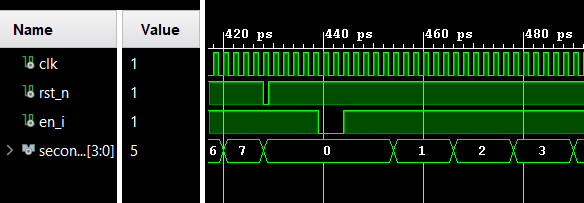
\includegraphics[width=13cm]{{images/sim_step2.2.png}}
    \centering
    \caption{This is the simulation of step 2}
\end{figure}

\begin{figure}[h]
    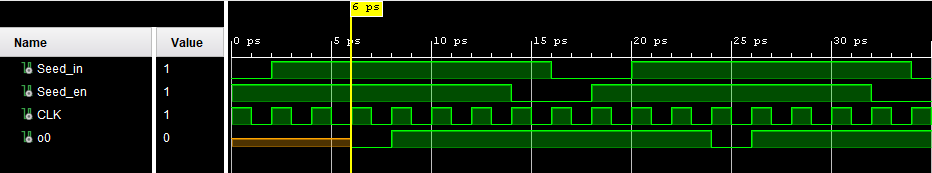
\includegraphics[width=13cm]{{images/sim_step3.png}}
    \centering
    \caption{This is the simulation of step 3}
\end{figure}

\begin{figure}[h]
    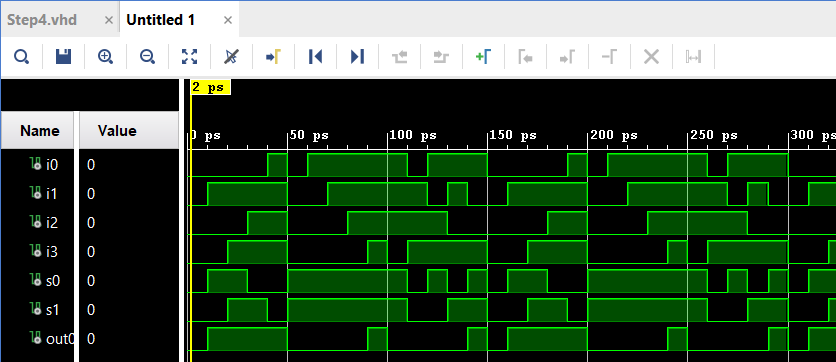
\includegraphics[width=13cm]{{images/sim_step4.png}}
    \centering
    \caption{This is the simulation of step 4, clock changes every 1ps so period of 2ps between every Rising edge.}
\end{figure}


\end{document}
